\documentclass{Notes}

\begin{document}

\tableofcontents

\chapter{Background}

Electrowetting-on-dielectric (EWOD)–based digital microfluidics (DMF) enables programmable manipulation of discrete droplets—such as dispensing, transport, merging, and splitting—using electric fields on a flat substrate as illustrated in Figure \ref{dmf_example}\subref{dmf_example}, unlike traditional continuous-flow microfluidics. This eliminates the need for mechanical components like micro-pumps or valves as shown in Figure \ref{dmf_example} \subref{microfluidics_example}. The underlying principle is governed by the Young–Lippmann equation, which relates voltage to contact angle modulation \cite{kimPCBbasedDigitalMicrofluidic2024}.

\begin{figure}[h!]
\centering
\begin{subfigure}[b]{0.49\linewidth}
\centering
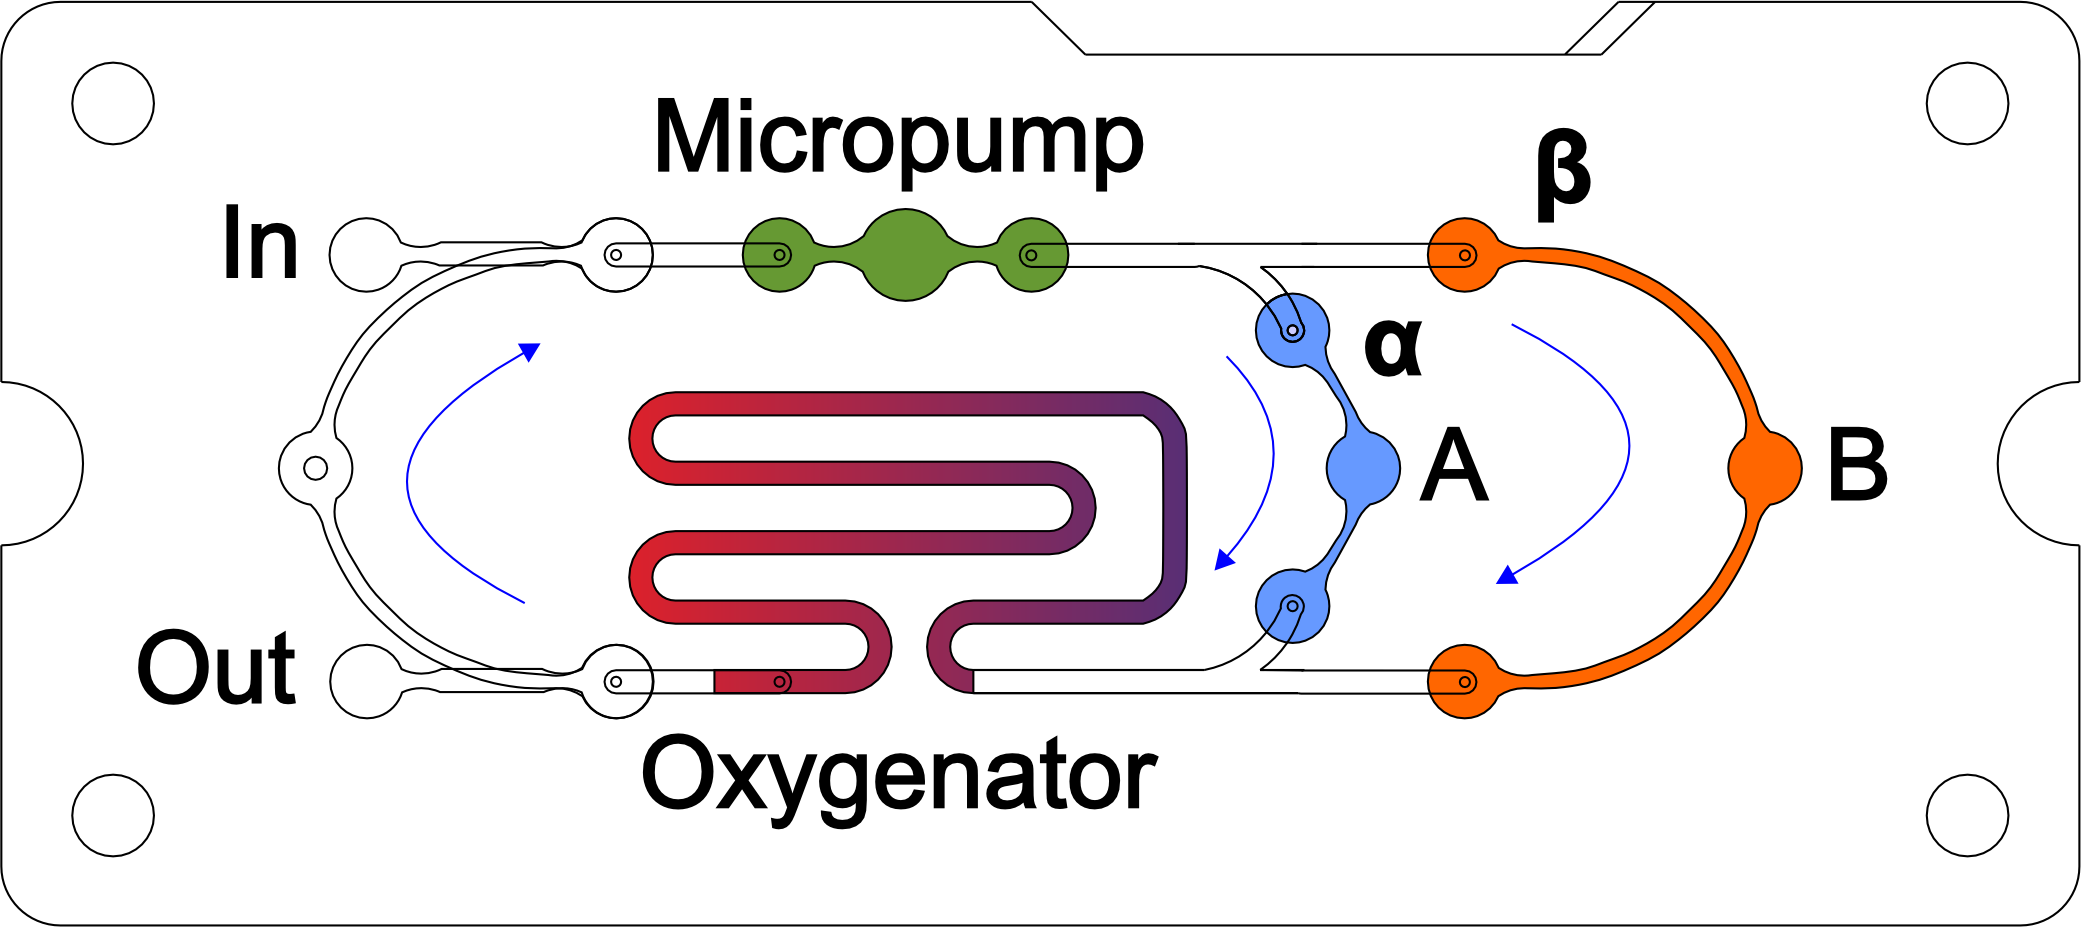
\includegraphics[width=\linewidth]{ExampleMicrofluidics.png}
\caption{}
\label{microfluidics_example}
\end{subfigure}
\begin{subfigure}[b]{0.49\linewidth}
\centering
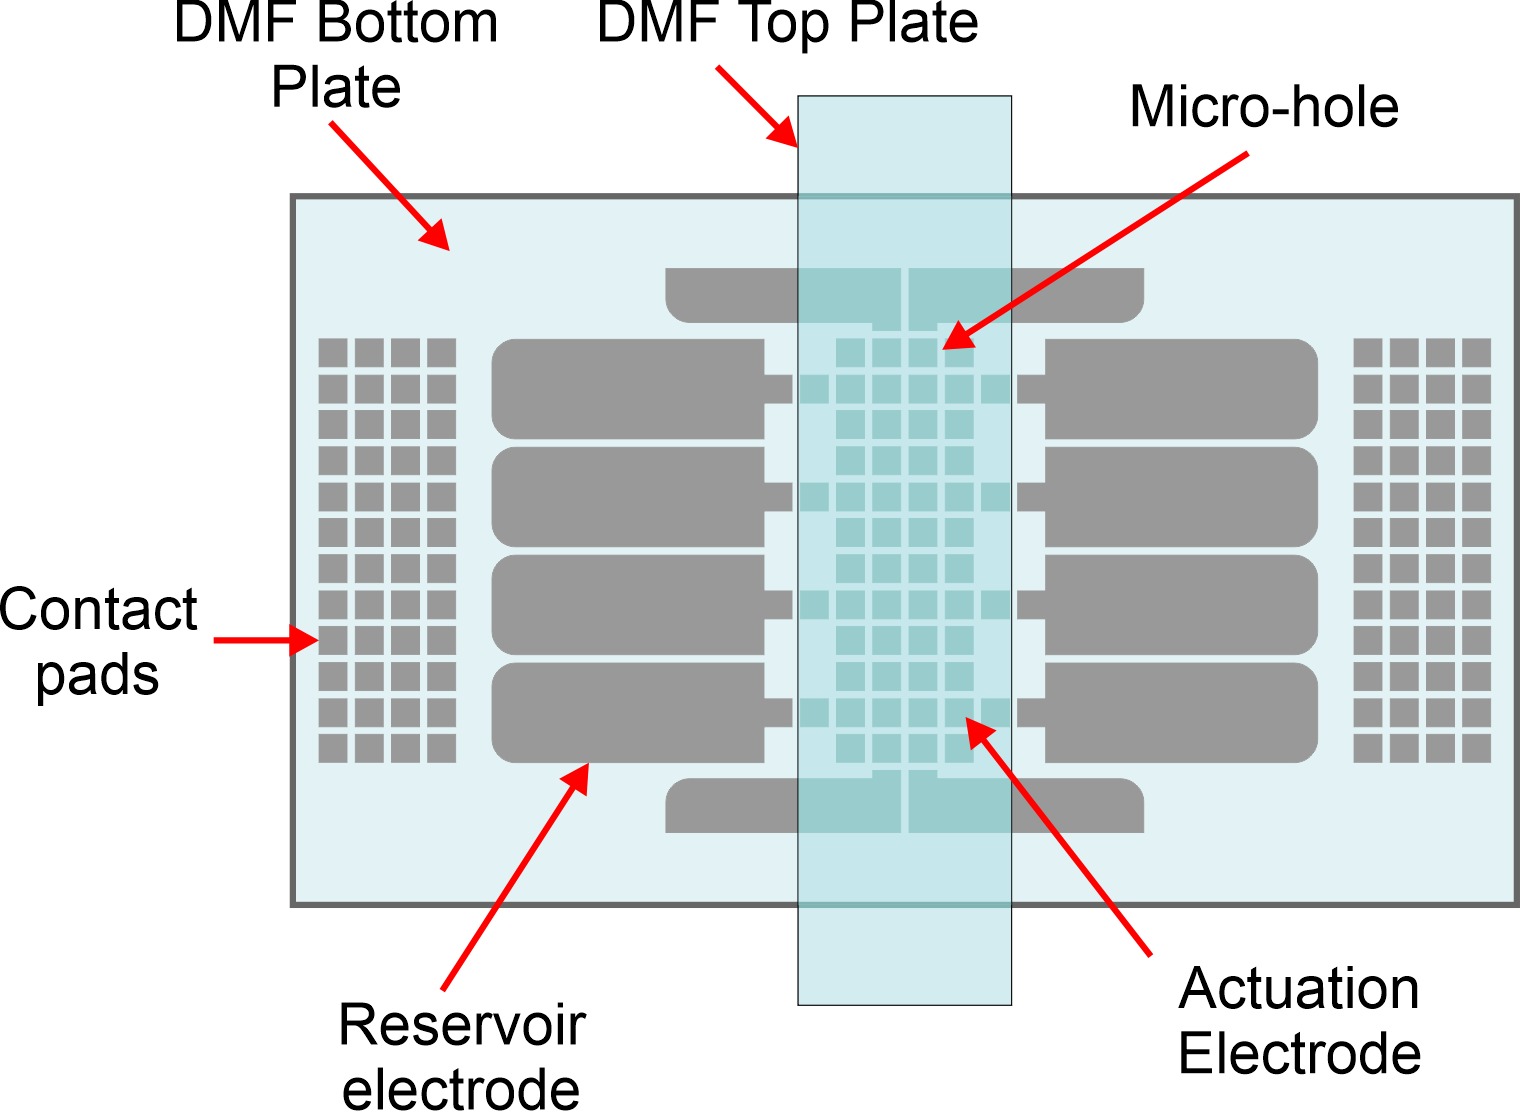
\includegraphics[width=\linewidth]{ExampleDMF.png}
\caption{}
\label{dmf_example}
\end{subfigure}
\caption{Comparison between \subref{microfluidics_example} conventional microfluidics (adapted from \cite{busekDesignCharacterizationModeling2016}) and \subref{dmf_example} EWOD-DMF device (adapted from \cite{pengAllinOneDigitalMicrofluidics2023}).}
\label{microfluidics_vs_dmf}
\end{figure}

Conventional EWOD-DMF systems are typically fabricated on glass or silicon using cleanroom processes \cite{vafaieNumericalSimulationEWOD2019}, which, while precise, are expensive and integration-limited. PCBs present a cost-effective, scalable alternative with mature fabrication methods, multilayer routing, and easy integration with control electronics \cite{jiangongDirectreferencingTwodimensionalarrayDigital2008,sukthangRapidFabricationCloseTyped2020,yiDesignOpenElectrowetting2020}.

\chapter{Methods}

% Bibliography
\backmatter
\bibliographystyle{IEEEtran}
\bibliography{Literature}

\end{document}
